%======================================================================
\section{Fundamentos de optimización}\label{sec:optimizacion}
%======================================================================
Esta sección reúne los conceptos de optimización que usa el resto del documento, desde lo más
básico. Las referencias generales son Nocedal y Wright~\cite{nocedal2006}, para la optimización
no lineal, y Boyd y Vandenberghe~\cite{boyd2004}, para la optimización convexa.

\subsection{Qué es un problema de optimización}
Un problema de optimización tiene tres ingredientes:
\begin{itemize}
  \item \textbf{variables de decisión} $z\in\mathbb R^n$: lo que se elige (aquí, los 26
        caudales del ACS, y a veces también los estados);
  \item \textbf{función objetivo} o costo $\phi(z)$: lo que se quiere hacer pequeño;
  \item \textbf{restricciones}: igualdades $c(z)=0$ y desigualdades $g(z)\le0$ que definen el
        \emph{conjunto factible} $\mathcal F=\{z:\ c(z)=0,\ g(z)\le0\}$.
\end{itemize}
Se escribe $\min_{z\in\mathcal F}\phi(z)$. Un problema es \emph{lineal} si el costo y las
restricciones son lineales; \emph{cuadrático} (QP) si el costo es cuadrático y las restricciones
lineales; y \emph{no lineal} (NLP) en el caso general.

\subsection{Mínimo local, mínimo global y convexidad}
\begin{definicion}[Mínimos local y global]
$z^\star\in\mathcal F$ es un \emph{mínimo global} si $\phi(z^\star)\le\phi(z)$ para todo
$z\in\mathcal F$. Es un \emph{mínimo local} si la desigualdad se cumple sólo para los $z$
factibles de algún entorno de $z^\star$.
\end{definicion}
\noindent Los métodos numéricos con derivadas son \emph{locales}: miran el costo cerca del
punto actual y bajan. Encuentran un mínimo local, pero no saben si hay otro mejor más lejos
(figura~\ref{fig:gap}). La propiedad que elimina esa incertidumbre es la convexidad.

\begin{definicion}[Convexidad]
Un conjunto $\mathcal F$ es convexo si el segmento entre dos de sus puntos está contenido en
él. Una función $\phi$ es convexa si
$\phi(\theta z+(1-\theta)w)\le\theta\phi(z)+(1-\theta)\phi(w)$ para todo $\theta\in[0,1]$: su
gráfico queda por debajo de cualquier cuerda. Si $\phi$ es dos veces diferenciable, es convexa
si y sólo si su hessiana $\nabla^2\phi$ es semidefinida positiva en todo punto.
\end{definicion}

\begin{proposicion}[En un problema convexo, todo mínimo local es global]\label{prop:convexo}
Si $\mathcal F$ y $\phi$ son convexos, todo mínimo local de $\phi$ en $\mathcal F$ es global.
\end{proposicion}
\begin{proof}
Sea $z^\star$ un mínimo local y supóngase que existe $w\in\mathcal F$ con $\phi(w)<\phi(z^\star)$.
Para $\theta\in(0,1)$, el punto $z_\theta=(1-\theta)z^\star+\theta w$ es factible por convexidad
de $\mathcal F$, y $\phi(z_\theta)\le(1-\theta)\phi(z^\star)+\theta\phi(w)<\phi(z^\star)$. Como
$z_\theta\to z^\star$ cuando $\theta\to0$, hay puntos arbitrariamente cerca de $z^\star$ con
menor costo, lo que contradice que sea un mínimo local.
\end{proof}

\begin{figure}[H]\centering
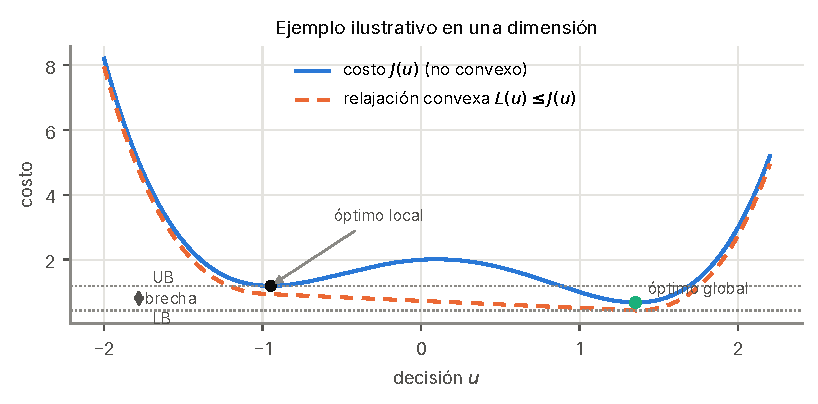
\includegraphics[width=\linewidth]{figures/did_gap.pdf}
\caption{Ejemplo ilustrativo en una dimensión. El costo $J$ (azul) no es convexo y tiene dos
mínimos. Un método local que arranque a la izquierda se detiene en el mínimo local, cuyo costo
es una cota superior (UB) del óptimo. Una función convexa $L\le J$ (naranja) tiene un único
mínimo, que es una cota inferior (LB). El óptimo global está atrapado entre UB y LB; la
diferencia es la \emph{brecha de optimalidad} (sección~\ref{sec:certteoria}).}
\label{fig:gap}
\end{figure}

\subsection{Condiciones de optimalidad}
\paragraph{En una variable sin restricciones.} En un mínimo interior, la derivada se anula,
$\phi'(z^\star)=0$: es la condición necesaria de \emph{primer orden}. Pero también se anula en
máximos y en puntos de inflexión. Si además $\phi''(z^\star)>0$, la función es localmente una
parábola hacia arriba y $z^\star$ es un mínimo local estricto: es la condición suficiente de
\emph{segundo orden}.

\paragraph{Con cotas.} Si $z$ debe estar en $[\ell,\upsilon]$ y el mínimo está en la cota
superior $z^\star=\upsilon$, la derivada no tiene por qué anularse: basta que sea negativa, porque
el costo bajaría si se pudiera seguir subiendo $z$, y la cota lo impide. Ese valor
$\mu=-\phi'(\upsilon)\ge0$ es el \emph{multiplicador} de la cota: mide cuánto bajaría el costo si
la cota se aflojara un poco. Ésta es la situación del ACS en 1161~s, donde el caudal óptimo es
el máximo permitido.

\paragraph{El caso general: condiciones KKT.} Para $\min\{\phi(z):c(z)=0,\ g(z)\le0\}$, en todo
mínimo local regular existen multiplicadores $\lambda$ y $\mu$ que cumplen las condiciones de
Karush--Kuhn--Tucker~\cite{nocedal2006}:
\[
\nabla\phi+\nabla c^\top\lambda+\nabla g^\top\mu=0,\quad c=0,\quad g\le0,\quad \mu\ge0,\quad \mu_ig_i=0.
\]
La primera ecuación es el equilibrio de fuerzas: el gradiente del costo se compensa con los
gradientes de las restricciones, ponderados por sus multiplicadores. La última, la
\emph{complementariedad}, dice que una desigualdad inactiva ($g_i<0$) tiene multiplicador
nulo. Las KKT son necesarias, pero no suficientes, y por eso hace falta una condición de
segundo orden.

\begin{proposicion}[Condición suficiente de mínimo local con cotas de caja]\label{prop:sosc}
Sea $J$ dos veces diferenciable y $u^\star\in[\ell,\upsilon]$. Supóngase que (i)
$\partial J/\partial u_k=0$ en las componentes libres ($\ell_k<u^\star_k<\upsilon_k$);
(ii) $\partial J/\partial u_k<0$ si $u^\star_k=\upsilon_k$ y $\partial J/\partial u_k>0$ si
$u^\star_k=\ell_k$ (complementariedad estricta); (iii) la hessiana restringida a las
componentes libres es definida positiva. Entonces $u^\star$ es un mínimo local estricto.
\end{proposicion}
\begin{proof}
Sea $u=u^\star+v$ factible y pequeño. Las componentes activas sólo pueden moverse hacia el
interior, y por (ii) el término lineal $\nabla J^\top v$ es estrictamente positivo si alguna de
ellas se mueve, y domina al término cuadrático para $v$ pequeño. Si sólo se mueven las libres,
el término lineal es nulo por (i), y por (iii)
$J(u)-J(u^\star)=\tfrac12v^\top\nabla^2J\,v+o(\|v\|^2)>0$.
\end{proof}

\subsection{Métodos con derivadas: Newton y punto interior}
\paragraph{El método de Newton.} Para resolver $\nabla\phi(z)=0$, Newton aproxima $\phi$ por su
expansión de Taylor de segundo orden en el punto actual y salta al mínimo de esa parábola:
\[
z^{(i+1)}=z^{(i)}-\big[\nabla^2\phi(z^{(i)})\big]^{-1}\nabla\phi(z^{(i)}).
\]
Cerca de un mínimo con hessiana definida positiva, el error se eleva al cuadrado en cada
iteración (convergencia \emph{cuadrática}): si una iteración tiene un error de $10^{-3}$, la
siguiente tiene uno del orden de $10^{-6}$. Por eso unas pocas iteraciones bastan. El precio es
que hacen falta primeras y segundas derivadas.

\paragraph{Método de punto interior.} Las desigualdades complican Newton, porque no se sabe de
antemano cuáles estarán activas. Los métodos de punto interior las reemplazan por una
\emph{barrera logarítmica}~\cite{nocedal2006}:
\[
\min_z\ \phi(z)-\mu_b\sum_i\ln\big(-g_i(z)\big),\qquad \mu_b\to0 .
\]
La barrera vale infinito en el borde del conjunto factible y mantiene los iterados en su
interior. Para cada $\mu_b$ se resuelve el problema con pasos de Newton, y $\mu_b$ se reduce
hacia cero. En una variable con la cota $z\le\upsilon$, por ejemplo, el término
$-\mu_b\ln(\upsilon-z)$ empuja a $z$ lejos de $\upsilon$, con una fuerza que se debilita a
medida que $\mu_b\to0$, hasta que el iterado puede apoyarse en la cota. \textbf{Ipopt}, el solver
que usa este trabajo para los problemas no lineales, es un método de punto interior primal-dual
con búsqueda lineal de filtro~\cite{wachter2006}. Para problemas no convexos garantiza un
mínimo local, no global.

\subsection{Cómo se obtienen las derivadas: diferenciación automática}
Hay tres maneras de obtener derivadas:
\begin{enumerate}
  \item \textbf{Diferencias finitas}: $\phi'(z)\approx(\phi(z+\varepsilon)-\phi(z-\varepsilon))/(2\varepsilon)$.
        Es simple, pero tiene un compromiso. Con $\varepsilon$ grande hay error de truncamiento;
        con $\varepsilon$ pequeño, error de redondeo. Además, cada derivada parcial cuesta dos
        evaluaciones.
  \item \textbf{Derivación simbólica}: derivar las fórmulas a mano o con un programa de
        álgebra. Es exacta, pero las expresiones crecen sin control en un modelo de 17
        ecuaciones.
  \item \textbf{Diferenciación automática} (AD)~\cite{griewank2008}: el programa que evalúa
        $\phi$ se ejecuta con un tipo de número extendido que lleva, junto a cada valor, su
        derivada. Aplicando la regla de la cadena operación por operación, el resultado es
        exacto hasta el redondeo.
\end{enumerate}

\begin{ejemplo}[Números duales]\label{ej:duales}
Un número dual es $a+b\,\epsilon$ con $\epsilon^2=0$. Si se evalúa una función en $z+\epsilon$,
el coeficiente de $\epsilon$ es su derivada: $f(z+\epsilon)=f(z)+f'(z)\,\epsilon$. Por ejemplo,
para $f(z)=z^2\sin z$ en $z=2$:
\[
(2+\epsilon)^2=4+4\epsilon,\qquad \sin(2+\epsilon)=\sin2+\cos2\,\epsilon,
\]
\[
(4+4\epsilon)(\sin2+\cos2\,\epsilon)=4\sin2+(4\sin2+4\cos2)\,\epsilon,
\]
y en efecto $f'(2)=2\cdot2\sin2+2^2\cos2=4\sin2+4\cos2$. Ninguna fórmula de la derivada se
escribió: salió de propagar $\epsilon$ por las operaciones.
\end{ejemplo}
\noindent Esto es la \emph{diferenciación automática en modo directo}, que implementa
ForwardDiff~\cite{revels2016} en Julia~\cite{bezanson2017}. Con un dual por variable de entrada
se obtiene el gradiente o el jacobiano completo. Anidando duales dentro de duales se obtienen
segundas derivadas. JuMP~\cite{dunning2017}, el lenguaje de modelado que se usa para escribir los
problemas, calcula internamente el gradiente y la hessiana exactos de la función lagrangiana
para Ipopt.

\subsection{Métodos sin derivadas}
Cuando la función es una caja negra, o es discontinua, se usan métodos que sólo la evalúan.
Los cuatro que aparecen en este documento son:
\begin{itemize}
  \item \textbf{Luus--Jaakola}: búsqueda aleatoria con región que se contrae~\cite{luus1973}
        (sección~\ref{sec:actual});
  \item \textbf{algoritmo genético}: población que evoluciona por selección, cruce y
        mutación~\cite{goldberg1989};
  \item \textbf{evolución diferencial} (DE): cada candidato se perturba con la diferencia
        entre otros dos de la población~\cite{storn1997}. Se usa en este trabajo como
        ``adversario'', para buscar un óptimo mejor que el de Ipopt;
  \item \textbf{enjambre de partículas} (PSO), que usan Liu et al.\ para ajustar el controlador
        PI~\cite{kennedy1995,liu2021}.
\end{itemize}

\begin{table}[H]\centering\small
\begin{tabularx}{\linewidth}{@{}l Y Y@{}}\toprule
& Con derivadas (Newton, punto interior) & Sin derivadas (LJ, GA, DE, PSO)\\\midrule
Qué necesita & Valor, gradiente y hessiana & Sólo el valor\\
Evaluaciones típicas & Decenas de iteraciones & Cientos a decenas de miles\\
Resultado & Mínimo local preciso, con certificado (KKT) & Buena solución aproximada, sin certificado\\
Reproducibilidad & Determinista & Depende de la semilla aleatoria\\
Funciona con discontinuidades & Mal & Bien\\
Escala con la dimensión & Bien (cientos o miles de variables) & Mal (la búsqueda se vuelve ciega)\\\bottomrule
\end{tabularx}
\caption{Métodos con y sin derivadas.}
\end{table}

\takeaway{\textbf{Para recordar.} Un método con derivadas encuentra un mínimo local de forma
rápida, precisa y reproducible, pero necesita una función suave y sus derivadas, que la
diferenciación automática obtiene de forma exacta. Un método sin derivadas sólo necesita
evaluar la función, pero cuesta muchas más evaluaciones y no garantiza nada. Ninguno de los
dos, por sí solo, garantiza el óptimo \emph{global} de un problema no convexo.}
